\section{Introduction}
\frame{\tableofcontents[currentsection, hideothersubsections]}

\begin{frame}
\frametitle{Keyword definitions}
\textbf{Planning:} sequential decision making
\vspace{10mm}
\pause

\begin{columns}
  \column{0.5\textwidth}
    \begin{figure}
        \centering
        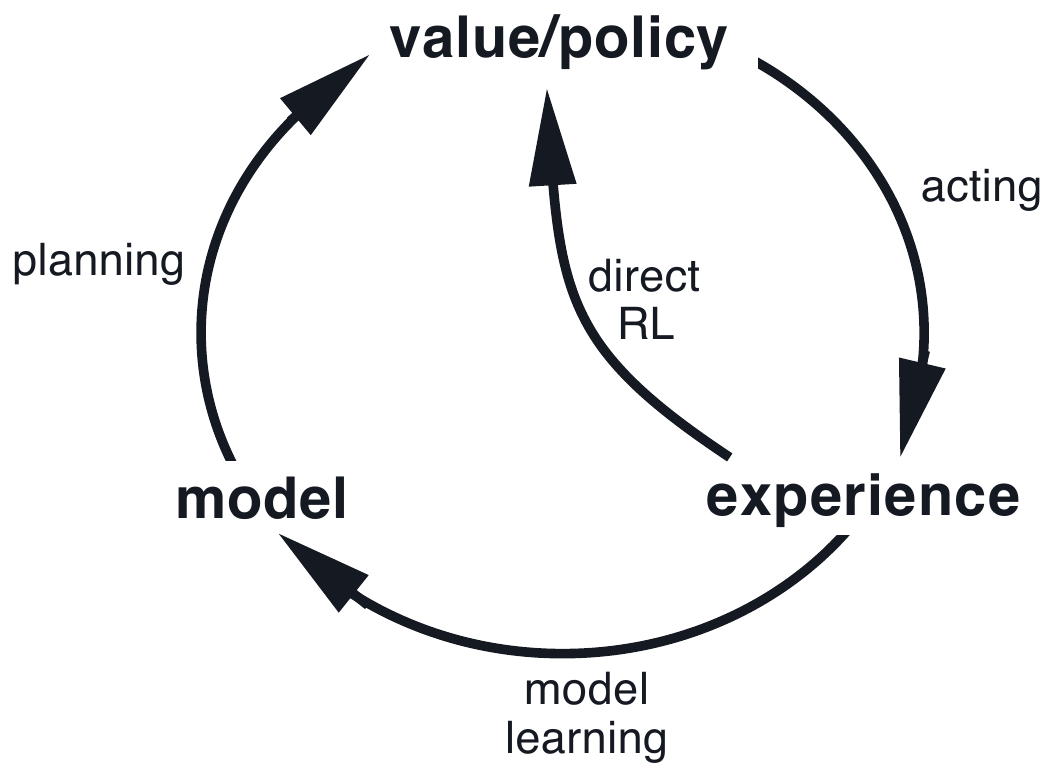
\includegraphics[scale=0.2]{planning_learning}
    \end{figure}
  \column{0.5\textwidth}
    \begin{figure}
        \centering
        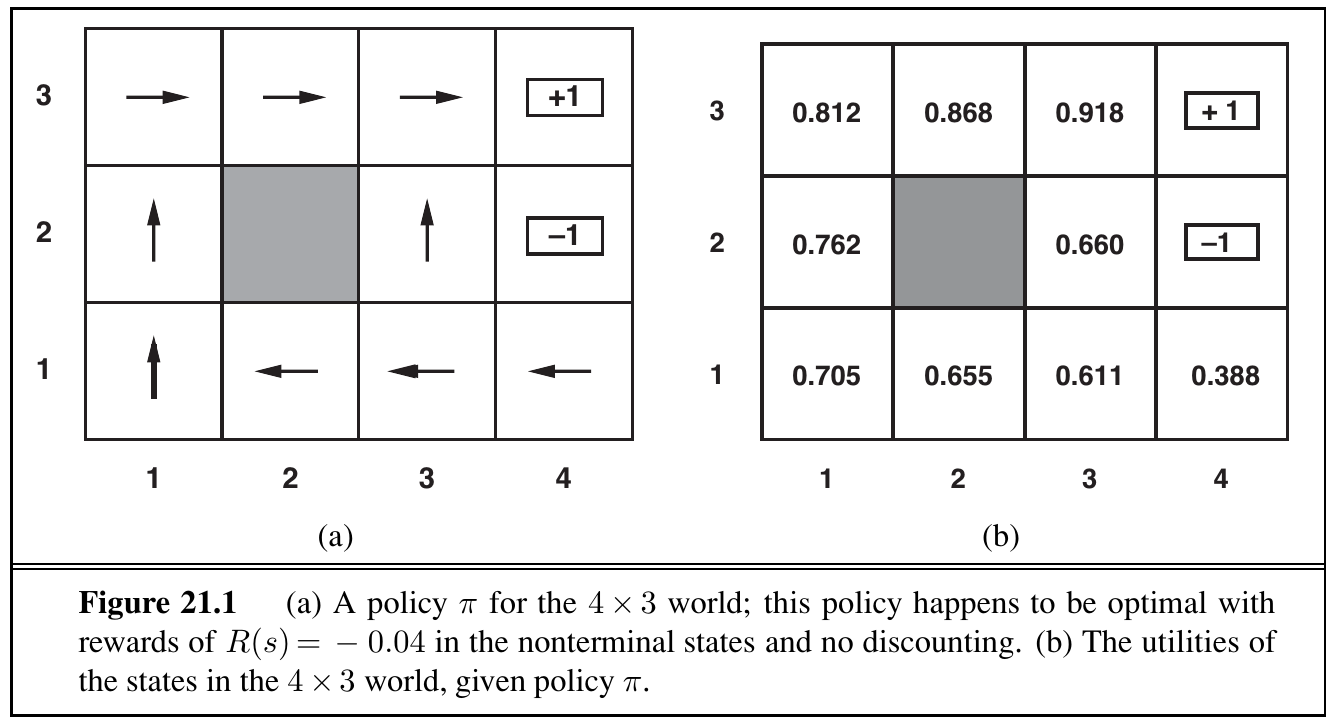
\includegraphics[scale=0.175]{policy_grid_world_aima_p832}
    \end{figure}
\end{columns}
\end{frame}

\begin{frame}
\frametitle{Keyword definitions}
\textbf{POMDP:} Partially Observable MDP
\pause

\begin{columns}
  \column{0.5\textwidth}
    \begin{figure}
        \centering
        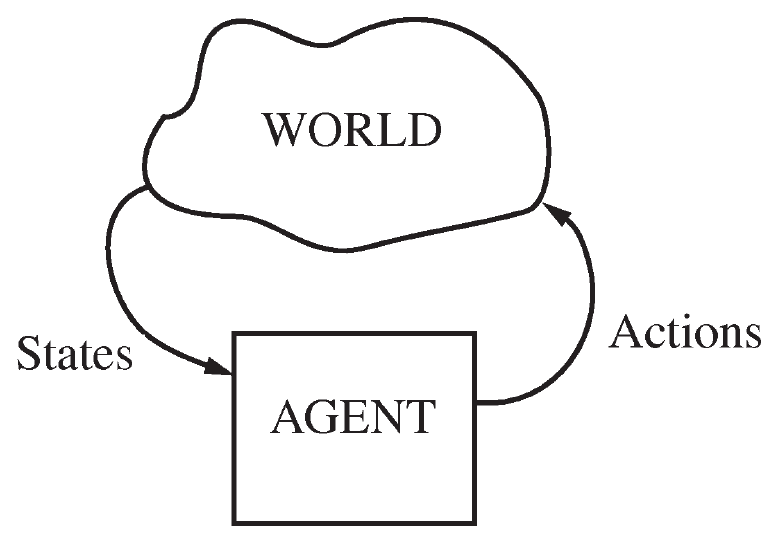
\includegraphics[scale=0.31]{mdp_agent}
        \caption{An MDP Agent}
    \end{figure}
  \column{0.5\textwidth}
    \begin{figure}
        \centering
        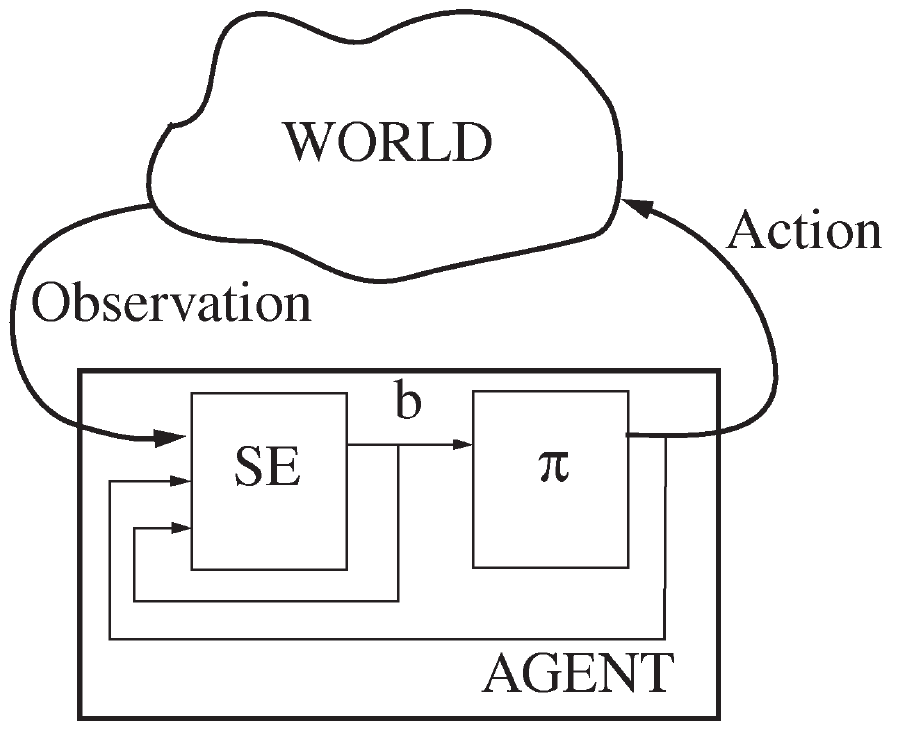
\includegraphics[scale=0.25]{pomdp_agent_leslie}
        \caption{A POMDP Agent}
    \end{figure}
\end{columns}

\end{frame}

\begin{frame}
\frametitle{Keyword definitions}
\textbf{Online:} planning is interleaved with execution, \\
to find a good \textbf{local policy} for the \textbf{current belief state} of the agent
\pause

\begin{figure}
    \centering
    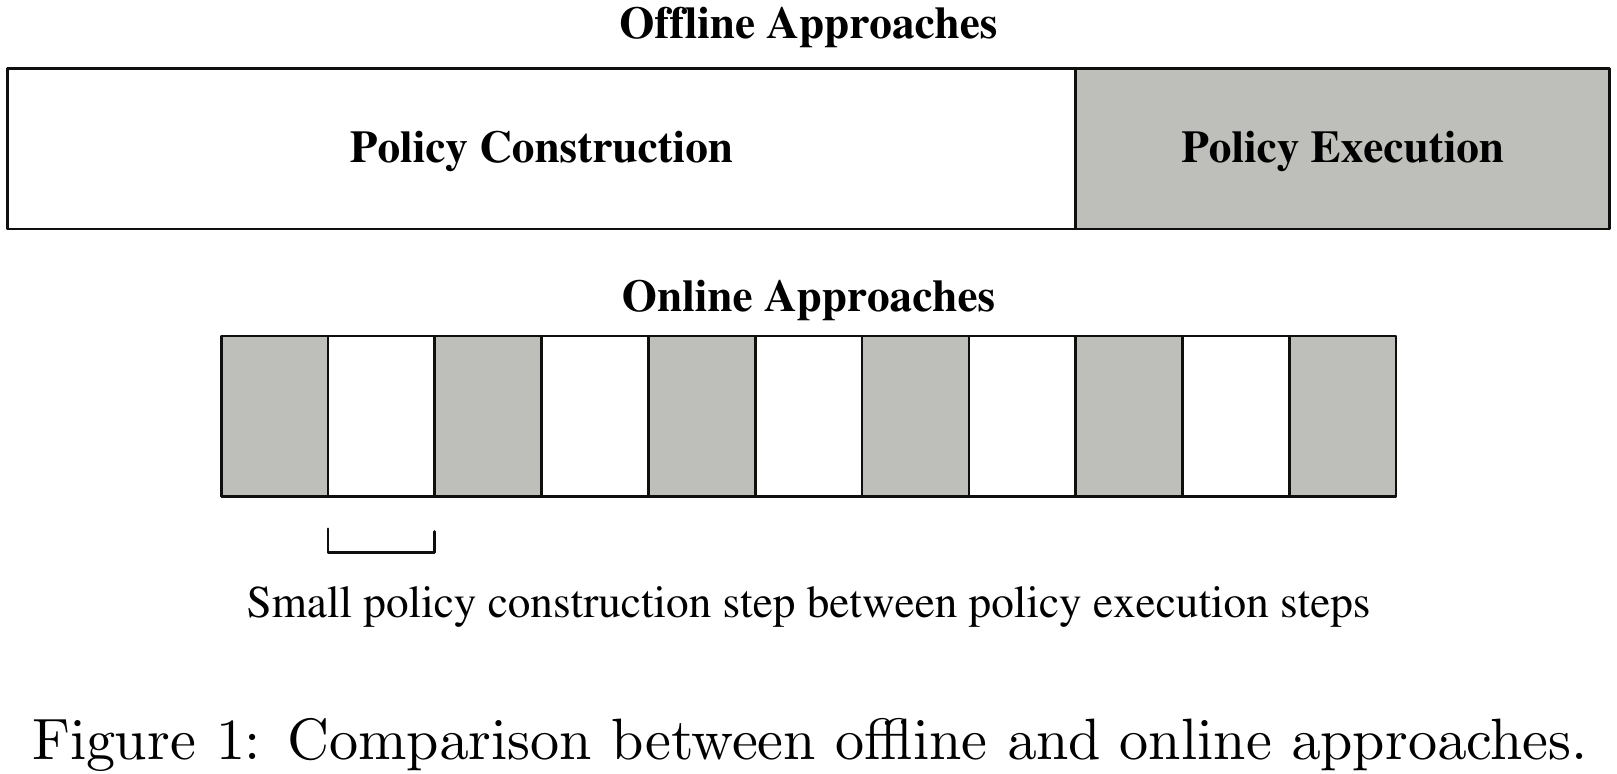
\includegraphics[scale=0.25]{online_offline_planning_ross}
\end{figure}
\pause

Note: offline planning is \textbf{not} applicable to large-size domains
\end{frame}

\begin{frame}
\frametitle{POMDP Formalities}
POMDP: $(S,A,T,Z,O,R,\gamma)$, with
\pause
\begin{itemize}
  \item $(S, A, T, R, \gamma)$ is the \textbf{underlying MDP} \pause
  \item $Z$ is the set of \textbf{all possible observations} \pause
  \item $O: S \times A \times Z \mapsto [0,1]$ is the \textbf{observation function}, where $O(s', a, z) = P(z|a, s')$
  gives the probability of observing $z$ if action $a$ is performed and the resulting state is $s'$
\end{itemize}
\end{frame}

\begin{frame}
\frametitle{Belief Tree: POMDP with 2 actions and 2 observations}
\begin{columns}
  \column{0.6\textwidth}
    \begin{figure}
        \centering
        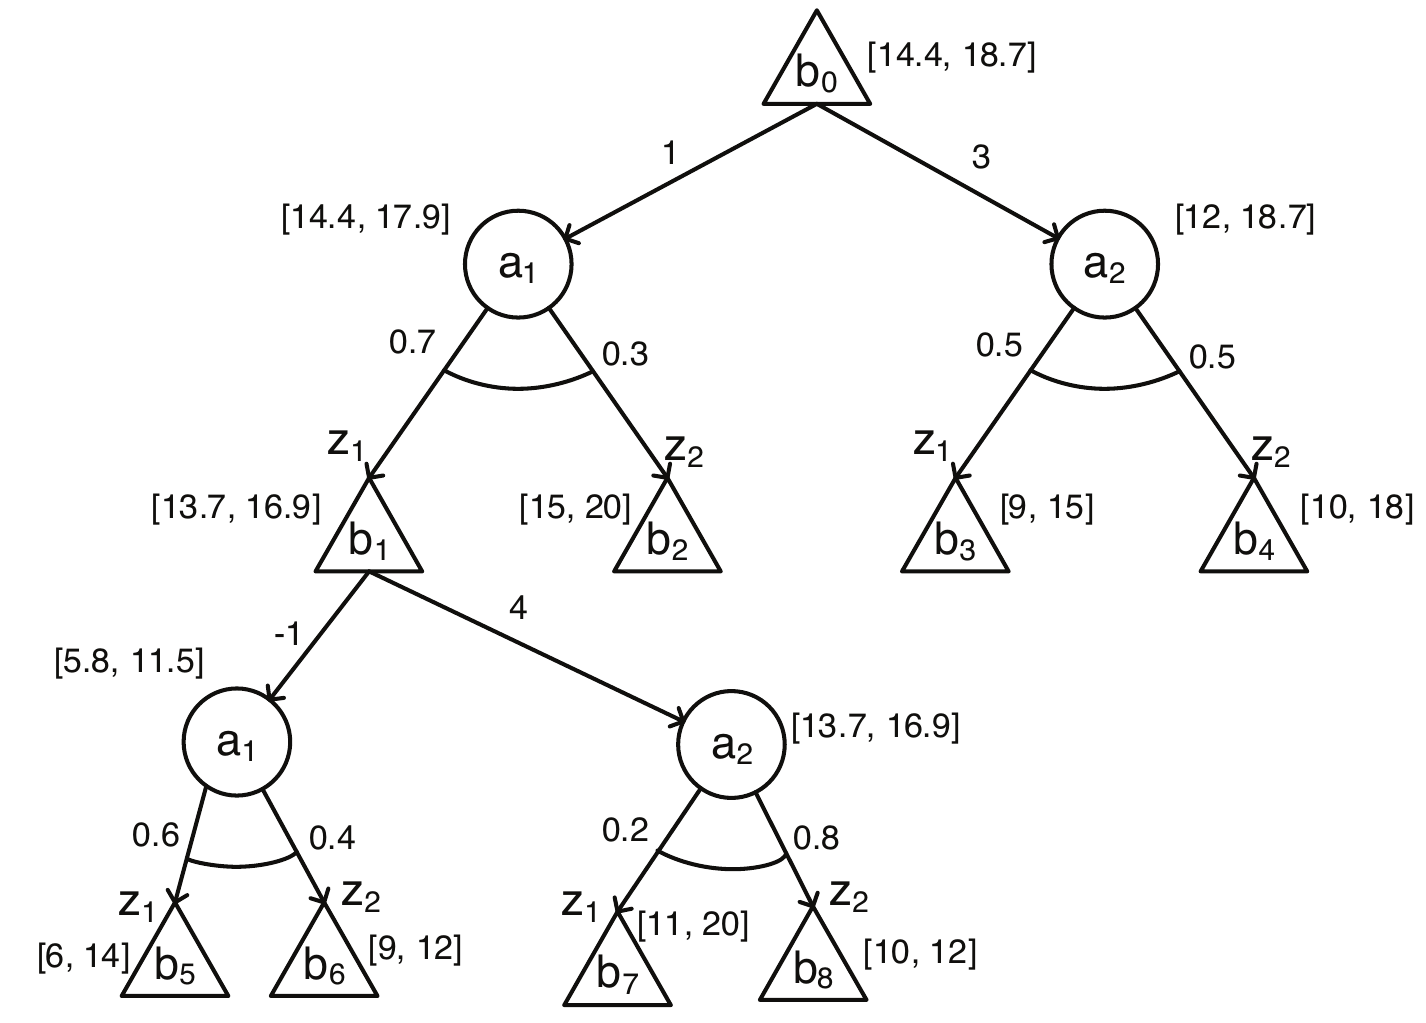
\includegraphics[scale=0.2]{and_or_tree}
    \end{figure}
  \column{0.4\textwidth}
    \begin{itemize}
        \item root node: current belief
        \item belief as OR-nodes \\
            (must choose an action)
        \item actions as AND-nodes \\
            {\scriptsize(must consider all observations)}
        \item $a_1$ in $b_1$ could be pruned
        \end{itemize}
\end{columns}
\end{frame}

\begin{frame}
\frametitle{Online Planning Framework: Sketch}
\begin{figure}
    \centering
    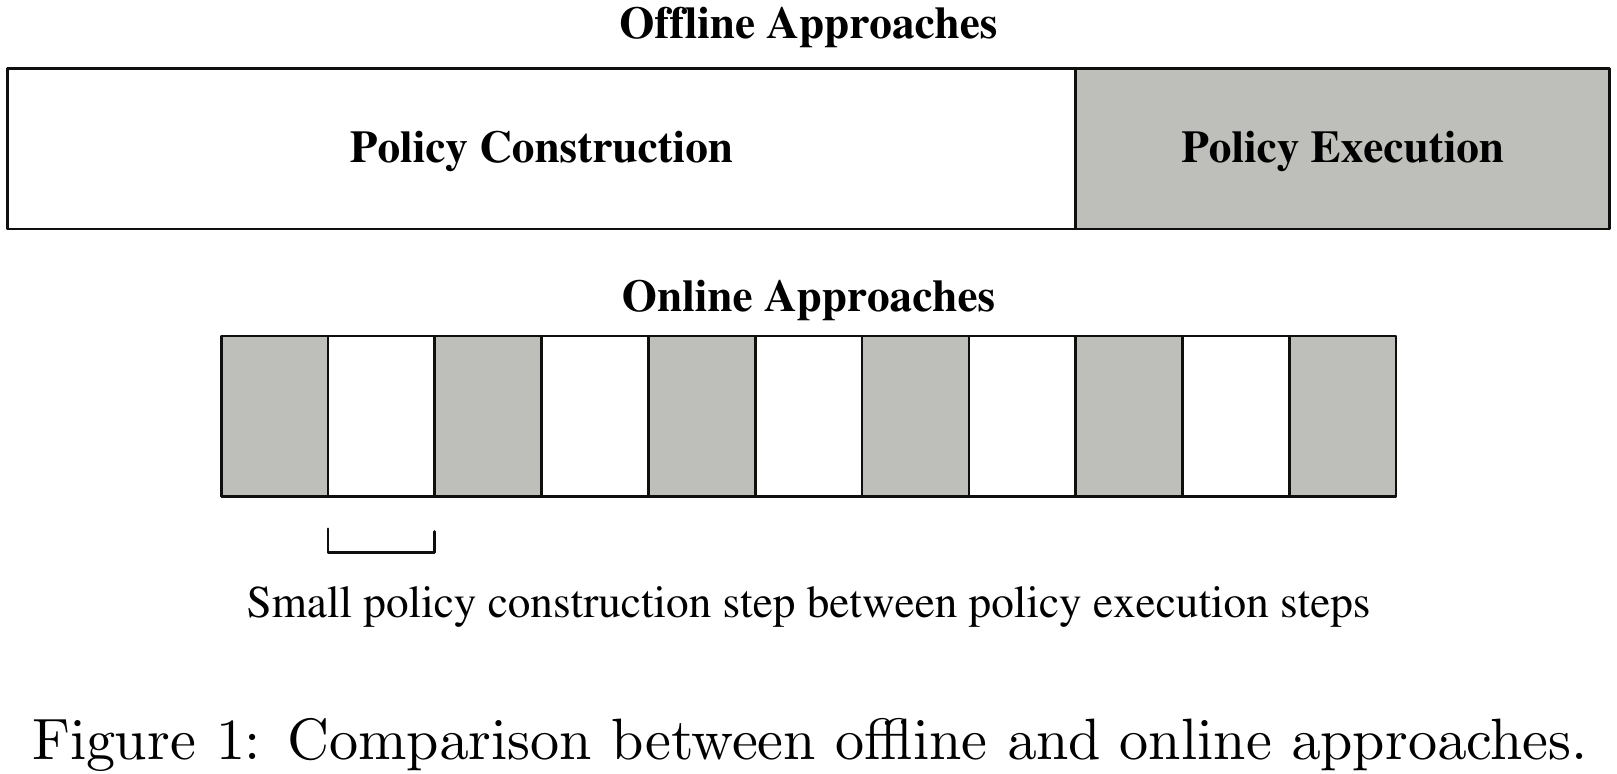
\includegraphics[scale=0.25,trim={0 3cm 0 7cm},clip]{online_offline_planning_ross}
\end{figure}

\begin{itemize}
    \item planning phase \pause
        \begin{itemize}
        \item given the current belief state \pause
        \item compute the best action to execute \pause
            \begin{itemize}
            \item build a tree of reachable belief states from the current belief \\
                by looking at several possible sequences of actions and observations
                \pause
            \item estimate the value of the current belief \\
                by propagating value estimates up from the fringe nodes, to their ancestors, all the way to the root
                \pause
            \end{itemize}
        \end{itemize}
    \item execution phase \pause
        \begin{itemize}
        \item execute the best action for the current belief \pause
        \item update the current belief and tree according to the observations
        \end{itemize}
\end{itemize}
\end{frame}

\begin{frame}
\frametitle{Online Planning Framework: Algorithm}
\begin{figure}
    \centering
    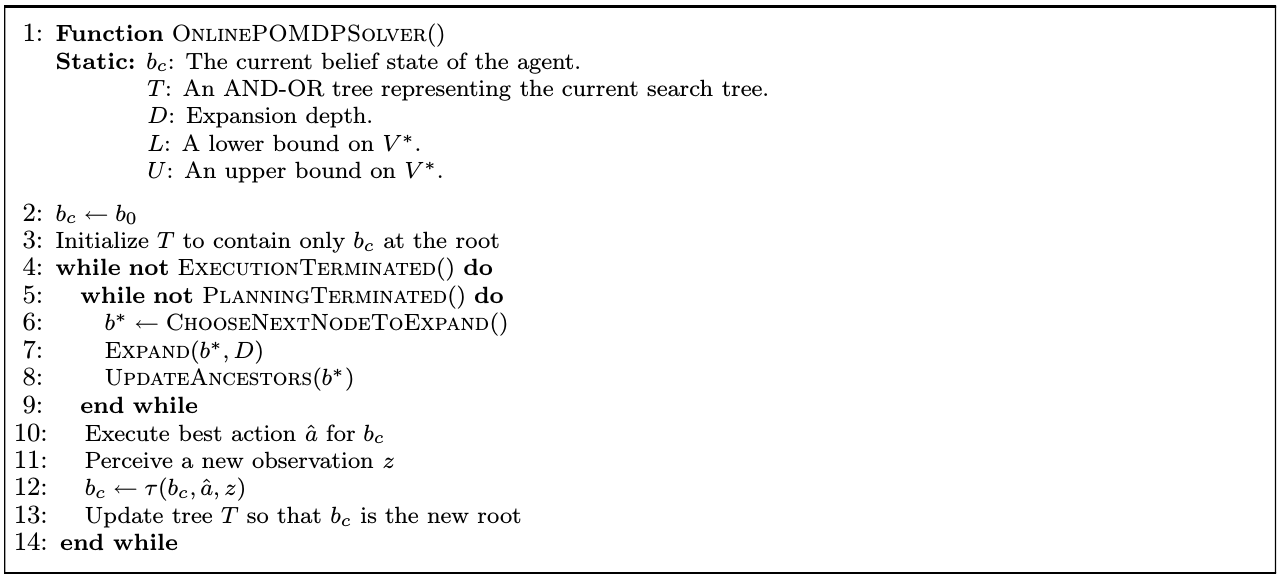
\includegraphics[scale=0.36]{online_framework}
\end{figure}

\begin{itemize}
\item planning phase: lines 5 to 9
\item execution phase: lines 10 to 13
\end{itemize}
\end{frame}